\documentclass[a4paper,12pt]{article}
\usepackage[a4paper, total={180mm, 272mm}]{geometry}

\usepackage{fontspec}
\setmainfont[Path=fonts/, Extension=.ttf]{ipaexm}

\setlength\parindent{3.5em}
\setlength\parskip{0em}
\renewcommand{\baselinestretch}{1.247}

\usepackage{eepic}
\usepackage{xcolor}

\usepackage{graphicx}
\graphicspath{{images/}}

\begin{document}

\thispagestyle{empty}

\Large
\noindent \\
HSV Noise Ino\medskip
\par
\normalsize
Add pixel noise to the Hue, Saturation, Value, and Alpha of the image.\par
It allows for adding noise to cell-like images, to blend in with the background.\\
\par
The Alpha channel will determine the strength of the noise. Therefore,\par
smooth edges will remain smooth.\par
The strength of the Alpha channel itself will also affect noise.\\
\par
When checking the results, sub-camera must not be used.\par
As the sub-camera uses a different input image range, the noise pattern will\par
be different.\\
\\
-{-}- \ Inputs \ -{-}-\\
Source\par
Connect the image to be processed.\\
Reference\par
Connect the reference image to assign the strength of the effect into each pixel.\\
\\
-{-}- \ Settings \ -{-}-\\
Hue\par
Specify the strength of the noise for the color tone (Hue).\par
Pixel value (8 or 16bits) specified as a value from 0 to 1.\par
Minimum value is 0, maximum value is 1.\par
When it is 0, no noise will be applied to the hue.\par
The default value is 0.025.\\
\\
Saturation\par
Specify the strength of the noise for the chroma (Saturation).\par
Pixel value (8 or 16bits) specified as a value from 0 to 1.\par
Minimum value is 0, maximum value is 1.\par
When it is 0, no noise will be applied to the chroma (Saturation).\par
The default value is 0.0.
\\
Value\par
Specify the strength of the noise for the Value.\par
Pixel value (8 or 16bits) specified as a value from 0 to 1.\par
Minimum value is 0, maximum value is 1.\par
When it is 0, no noise will be applied to the Value.\par
The default value is 0.035.\\

\newpage

\thispagestyle{empty}

\ \vspace{-0.2em}
\par
\noindent Alpha\par
Specify the strength of the noise for the Alpha channel.\par
Pixel value (8 or 16bits) specified as a value from 0 to 1.\par
Minimum value is 0, maximum value is 1.\par
When it is 0, no noise will be applied to the Alpha channel.\par
The default value is 0.0.\\
\\
Seed\par
This value is used to determine the noise pattern to be applied to the image.\par
Specify an integer value greater than or equal to 0.\par
When this value is the same, it will produce the same pattern.\par
When this value is different, a different noise pattern will be produced.\par
The default value is 1.\\
\\
NBlur\par
It blurs the noise component, reducing the dots presence in the image.\par
Minimum value is 0, maximum value is 1.\par
Because it is calculated only in pixels adjacent to the dot,\par
it will feel like a very light blur.\par
When at 0, no blur will be applied; when at 1, it will apply an average of\par 
neighbor pixels.\par
The default value is 1.\\
\\
Limits\par
Adjusts the effect on the extremes (near 0 or 1) of Saturation, Value, and\par Alpha changes.\par
When noise is applied near 0 or 1, values less than 0 or greater than 1 could be\par generated, but since it cannot be expressed, they are truncated to 0 or 1\par 
respectively. This allows to compensate for the truncation.\par
-{-}> See Figure 1: \textquotedbl Noise effect adjustments at extremes values\textquotedbl.\par
-{-}> See Figure 2: \textquotedbl Illustration of noise change range at extreme values\textquotedbl.\\
\par
\noindent \ \ \, Effective\par
Determines the strength of the Limits effect.\par
When the value is at 0, it has no effect. The effect will be shown when values are\par 
greater than 0\par
A value of 1 will have the strongest effect.\par
The default value is 0.\\
\par

\newpage

\thispagestyle{empty}

\ \vspace{-0.2em}
\par
\noindent \ \ \, Center\par
Defines the center of the effect.\par
Allows to shift the range of the Limits effect, with more intensity at the\par 
extremes, and no intensity at its center.\par
The center value position will show no limiting effect.\par
The value must be between 0 and 1.\par
If is 0, Limits effect will have no effect for pixel values of 0.\par
If is 1, Limits effect will have no effect for pixel values of 1.\par
The default Center value is 0.5.\\
\par
\noindent \ \ \, Type\par
Select the Type of the effect.\par
When \textquotedbl Keep Noise\textquotedbl\ is selected, the overall noise range is\par 
shifted, maintaining its width, and reducing the contrast of the image.\par
When \textquotedbl Keep Contrast\textquotedbl\ is selected, the noise range width is\par 
reduced only at the extremes, to maintain the contrast of the image.\par
The default setting is \textquotedbl Keep Noise\textquotedbl .\\
\\
Premultiplied\par
When ON, the image will be processed as if having a Premultiplied Alpha channel\par 
(Alpha value already multiplied by RGB channels).\par
If image is not premultiplied, the image may not look correct.\par
The default setting is ON.\\
\\
Reference\par
Specify which channel to use from the image connected to the Reference port to\par 
drive the intensity of the effect.\par
Choose from Red/Green/Blue/Alpha/Luminance.\par
Choose Nothing to disable the effect.\par
The default value is \textquotedbl Red\textquotedbl .

\newpage

\thispagestyle{empty}

\ \vspace{1.5em}
\par
\noindent \hskip 2.2em Figure 1 Noise effect adjustments at extremes values.\\[0.4em]
\par
\scriptsize
\noindent \hskip 3.4em Original\par
\noindent \hskip 3.4em Effective = 0\par
\noindent \hskip 3.4em Keep Noise\par
\noindent \hskip 3.4em Keep Contrast

\large
\noindent \begin{picture}(0,0)
\put(55.5,-6.5){
\includegraphics[width=29.6em, height=1em]{HSVNoiseInoNoiseEffectOriginal}}
\put(55.5,-22.5){
\includegraphics[width=29.6em, height=1em]{HSVNoiseInoNoiseEffectEffectiveZero}}
\put(55.5,-38.5){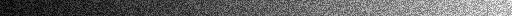
\includegraphics[width=29.6em, height=1em]{HSVNoiseInoNoiseEffectKeepNoise}}
\put(55.5,-54.5){
\includegraphics[width=29.6em, height=1em]{HSVNoiseInoNoiseEffectKeepContrast}}
\linethickness{0.01em}
\put(126,64){\line(-1,0){56}}
\put(126,53){\line(-1,0){14}}
\put(126,41){\line(-1,0){42}}
\put(126,29.5){\line(-1,0){28}}
\put(126,15){\line(-1,0){93}}
\put(126,64){\line(0,-1){49}}
\put(33,15){\line(0,-1){58}}
\put(33,0){\line(1,0){14}}
\put(47,0){\line(-3,2){6}}
\put(47,0){\line(-3,-2){6}}
\put(33,-14){\line(1,0){14}}
\put(47,-14){\line(-3,2){6}}
\put(47,-14){\line(-3,-2){6}}
\put(33,-28){\line(1,0){14}}
\put(47,-28){\line(-3,2){6}}
\put(47,-28){\line(-3,-2){6}}
\put(33,-43){\line(1,0){14}}
\put(47,-43){\line(-3,2){6}}
\put(47,-43){\line(-3,-2){6}}
\end{picture}\\[3.6em]

\normalsize
\noindent \hskip 2.2em Figure 2 Illustration of noise change range at extreme values.\\[0.5em]
\par
\footnotesize
\noindent \hskip 2.65em Effective = 0: \ \ Noise extreme values are cut. (default)

\large
\noindent \begin{picture}(0,0)
\linethickness{0.01em}
\put(54.5,-37){\line(0,1){8}}
\put(54.5,-37){\line(-2,3){3}}
\put(54.5,-37){\line(2,3){3}}
\put(482,-37){\line(0,1){8}}
\put(482,-37){\line(-2,3){3}}
\put(482,-37){\line(2,3){3}}
\put(54.5,-58){\line(0,1){6}}
\put(482,-58){\line(0,1){6}}

\put(27,-45.5){\line(1,0){56}}
\put(27,-45.5){\line(3,2){6}}
\put(27,-45.5){\line(3,-2){6}}
\put(83,-45.5){\line(-3,2){6}}
\put(83,-45.5){\line(-3,-2){6}}

\put(255,-45.5){\line(1,0){56}}
\put(255,-45.5){\line(3,2){6}}
\put(255,-45.5){\line(3,-2){6}}
\put(311,-45.5){\line(-3,2){6}}
\put(311,-45.5){\line(-3,-2){6}}

\put(455,-45.5){\line(1,0){56}}
\put(455,-45.5){\line(3,2){6}}
\put(455,-45.5){\line(3,-2){6}}
\put(511,-45.5){\line(-3,2){6}}
\put(511,-45.5){\line(-3,-2){6}}

\put(61,-67){\line(1,0){15}}
\put(61,-67){\line(3,2){6}}
\put(61,-67){\line(3,-2){6}}
\put(52,-70){\scriptsize{0}}
\put(78,-74){\footnotesize{Noise values of 0 or less, limited to 0}}

\put(471,-67){\line(-1,0){15}}
\put(471,-67){\line(-3,2){6}}
\put(471,-67){\line(-3,-2){6}}
\put(476,-70){\scriptsize{1.0}}
\put(312,-74){\footnotesize{Noise values of 1 or more, limited to 1}}

\linethickness{0.2em}
\put(54.5,-38){\line(1,0){428}}
\linethickness{2.8em}
\put(49,-1.5){\line(1,0){439}}
\linethickness{2.75em}
\color{lightgray}
\put(45.5,-1.5){\line(1,0){438}}
\put(51,-0.5){
\includegraphics[width=29.55em, height=1em]{HSVNoiseInoNoiseEffectOriginal}}
\put(51,-16.5){
\includegraphics[width=29.55em, height=1em]{HSVNoiseInoNoiseEffectEffectiveZero}}
\end{picture}\\[5.7em]

\footnotesize
\noindent \hskip 2.65em Keep Noise: \ \ Shift maintaining noise. Contrast is reduced. Noise position is shifted overall.

\large
\noindent \begin{picture}(0,0)
\linethickness{0.01em}
\put(255,-45.5){\line(1,0){56}}
\put(255,-45.5){\line(3,2){6}}
\put(255,-45.5){\line(3,-2){6}}
\put(311,-45.5){\line(-3,2){6}}
\put(311,-45.5){\line(-3,-2){6}}

\put(158,-60){\line(0,1){8}}
\put(158,-60){\line(-2,3){3}}
\put(158,-60){\line(2,3){3}}
\put(400,-60){\line(0,1){8}}
\put(400,-60){\line(-2,3){3}}
\put(400,-60){\line(2,3){3}}

\put(144,-68.5){\line(1,0){56}}
\put(144,-68.5){\line(3,2){6}}
\put(144,-68.5){\line(3,-2){6}}
\put(200,-68.5){\line(-3,2){6}}
\put(200,-68.5){\line(-3,-2){6}}

\put(357,-68.5){\line(1,0){56}}
\put(357,-68.5){\line(3,2){6}}
\put(357,-68.5){\line(3,-2){6}}
\put(413,-68.5){\line(-3,2){6}}
\put(413,-68.5){\line(-3,-2){6}}

\put(107,-83){\line(0,1){8}}
\put(107,-83){\line(-2,3){3}}
\put(107,-83){\line(2,3){3}}
\put(442,-83){\line(0,1){8}}
\put(442,-83){\line(-2,3){3}}
\put(442,-83){\line(2,3){3}}

\put(102,-91.5){\line(1,0){56}}
\put(102,-91.5){\line(3,2){6}}
\put(102,-91.5){\line(3,-2){6}}
\put(158,-91.5){\line(-3,2){6}}
\put(158,-91.5){\line(-3,-2){6}}

\put(392,-91.5){\line(1,0){56}}
\put(392,-91.5){\line(3,2){6}}
\put(392,-91.5){\line(3,-2){6}}
\put(448,-91.5){\line(-3,2){6}}
\put(448,-91.5){\line(-3,-2){6}}

\put(58,-106){\line(0,1){8}}
\put(58,-106){\line(-2,3){3}}
\put(58,-106){\line(2,3){3}}
\put(478.5,-106){\line(0,1){8}}
\put(478.5,-106){\line(-2,3){3}}
\put(478.5,-106){\line(2,3){3}}

\put(55,-114.5){\line(1,0){56}}
\put(55,-114.5){\line(3,2){6}}
\put(55,-114.5){\line(3,-2){6}}
\put(111,-114.5){\line(-3,2){6}}
\put(111,-114.5){\line(-3,-2){6}}

\put(427,-114.5){\line(1,0){56}}
\put(427,-114.5){\line(3,2){6}}
\put(427,-114.5){\line(3,-2){6}}
\put(483,-114.5){\line(-3,2){6}}
\put(483,-114.5){\line(-3,-2){6}}

\put(283,-106){\line(0,1){54}}
\put(267,-123){\scriptsize{separate}}

\linethickness{0.2em}
\put(54.5,-38){\line(1,0){428}}
\put(54.5,-61){\line(1,0){428}}
\put(54.5,-84){\line(1,0){428}}
\put(54.5,-107){\line(1,0){428}}
\linethickness{2.8em}
\put(49,-1.5){\line(1,0){439}}
\linethickness{2.75em}
\color{lightgray}
\put(45.5,-1.5){\line(1,0){438}}
\put(51,-0.5){
\includegraphics[width=29.55em, height=1em]{HSVNoiseInoNoiseEffectOriginal}}
\put(51,-16.5){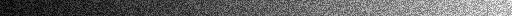
\includegraphics[width=29.55em, height=1em]{HSVNoiseInoNoiseEffectKeepNoise}}
\end{picture}\\[9.3em]

\footnotesize
\noindent \hskip 2.65em Keep Contrast: \ \ Noise width reduced at extremes. Contrast is maintained.

\large
\noindent \begin{picture}(0,0)
\linethickness{0.01em}
\put(255,-45.5){\line(1,0){56}}
\put(255,-45.5){\line(3,2){6}}
\put(255,-45.5){\line(3,-2){6}}
\put(311,-45.5){\line(-3,2){6}}
\put(311,-45.5){\line(-3,-2){6}}

\put(86,-60){\line(0,1){8}}
\put(86,-60){\line(-2,3){3}}
\put(86,-60){\line(2,3){3}}
\put(450,-60){\line(0,1){8}}
\put(450,-60){\line(-2,3){3}}
\put(450,-60){\line(2,3){3}}

\put(58,-68.5){\line(1,0){56}}
\put(58,-68.5){\line(3,2){6}}
\put(58,-68.5){\line(3,-2){6}}
\put(114,-68.5){\line(-3,2){6}}
\put(114,-68.5){\line(-3,-2){6}}

\put(423,-68.5){\line(1,0){56}}
\put(423,-68.5){\line(3,2){6}}
\put(423,-68.5){\line(3,-2){6}}
\put(479,-68.5){\line(-3,2){6}}
\put(479,-68.5){\line(-3,-2){6}}

\put(70,-83){\line(0,1){8}}
\put(70,-83){\line(-2,3){3}}
\put(70,-83){\line(2,3){3}}
\put(468,-83){\line(0,1){8}}
\put(468,-83){\line(-2,3){3}}
\put(468,-83){\line(2,3){3}}

\put(55,-91.5){\line(1,0){28}}
\put(55,-91.5){\line(3,2){6}}
\put(55,-91.5){\line(3,-2){6}}
\put(83,-91.5){\line(-3,2){6}}
\put(83,-91.5){\line(-3,-2){6}}

\put(454,-91.5){\line(1,0){28}}
\put(454,-91.5){\line(3,2){6}}
\put(454,-91.5){\line(3,-2){6}}
\put(482,-91.5){\line(-3,2){6}}
\put(482,-91.5){\line(-3,-2){6}}

\put(61,-106){\line(0,1){8}}
\put(61,-106){\line(-2,3){3}}
\put(61,-106){\line(2,3){3}}
\put(476.5,-106){\line(0,1){8}}
\put(476.5,-106){\line(-2,3){3}}
\put(476.5,-106){\line(2,3){3}}

\put(55,-114.5){\line(1,0){12}}
\put(55,-114.5){\line(3,2){6}}
\put(55,-114.5){\line(3,-2){6}}
\put(67,-114.5){\line(-3,2){6}}
\put(67,-114.5){\line(-3,-2){6}}

\put(471,-114.5){\line(1,0){12}}
\put(471,-114.5){\line(3,2){6}}
\put(471,-114.5){\line(3,-2){6}}
\put(483,-114.5){\line(-3,2){6}}
\put(483,-114.5){\line(-3,-2){6}}

\put(283,-106){\line(0,1){54}}
\put(267,-123){\scriptsize{separate}}

\linethickness{0.2em}
\put(54.5,-38){\line(1,0){428}}
\put(54.5,-61){\line(1,0){428}}
\put(54.5,-84){\line(1,0){428}}
\put(54.5,-107){\line(1,0){428}}
\linethickness{2.8em}
\put(49,-1.5){\line(1,0){439}}
\linethickness{2.75em}
\color{lightgray}
\put(45.5,-1.5){\line(1,0){438}}
\put(51,-0.5){
\includegraphics[width=29.55em, height=1em]{HSVNoiseInoNoiseEffectOriginal}}
\put(51,-16.5){
\includegraphics[width=29.55em, height=1em]{HSVNoiseInoNoiseEffectKeepContrast}}
\end{picture}

\end{document}